\section{Are there Grandmother Cells in CNNs? How distributed are the representations?}
\label{sec:grand-mother}
Neuroscientists have conjectured that cells in the human brain which only respond to very specific and complex visual stimulus (such as the face of one's grandmother) are involved in object recognition and termed them as Grandmother Cells (GMC) \cite{Barlow}, \cite{Grandmother}. Proponents of artificial neural networks have shown a great interest in reporting the presence of GMC like filters for specific object classes in their networks \cite{GoogleCat}. More recently, for understanding feature representations in CNN, \cite{DeConv}, \cite{Simonyan} presented methods for finding the optimal visual input for individual filters. Mathematically, this computation is expressed as finding the set of images $\mathcal{I}$ which maximally activate a single feature (i.e. find $i \in \mathcal{I}$ s.t. Feature-score(i) $\geq th$ $\forall i $, where $th$ is a threshold value). The distribution of class labels associated with this set of images ($\mathcal{I}$), defines the \textit{precision} of the feature. However, this distribution does not account for the \textit{recall}.  The presence/absence of GMC is a scientifically interesting question to pursue, but for recognition, we require features with both high precision and high recall. Consequently, we argue that if the goal is object recognition, then GMC for a particular object class should be interpreted as features with high AP and not just high precision. 
 
Further, prior to the work of \cite{Kriz}, the dominant approaches for image and scene classification were based on either representing images as a bag of local descriptors (or words) such as SIFT (BoW model, \cite{SPM}) or using mid-level patches \cite{Mid1}, \cite{Blocks}. The BoW feature representation is a distributed code (i.e. a single feature by itself is not discriminative, but a group of features taken together is.), whereas the problem of finding good mid-level patches is often posed as a greedy search for high recall discriminative templates. Mid-level patches are closer to the GMC-like representation. Given this, it is interesting to investigate the CNN features to find the kind of representations they employ.

We perform such analysis in two phases using conv-5 features. In the first phase, we directly address the question of finding GMC (section \ref{sub:class-specific-unit}) by computing AP of individual filters. Next, we determine the total number of filters required for achieving the same 

We divide our analysis into two parts. In sec \ref{sub:class-specific-unit} we try to address if there exist filters with very high precision (aka Grand-Mother cells) and in sec \ref{sub:how-many} we answer how many filters are required to discriminate a class. 

\subsection{Finding Grandmother Cells}
\label{sub:class-specific-unit}
%Precision for each filter from layer 5 is computed in a way analogous to entropy computation described in \ref{sub:def-ent}. In the final step instead of computing the entropy, we compute Prob(Class $|$ Filter Activity $\geq$ threshold). We define the selectivity of a filter as the area under the precision curve. 

For this computation we use ground truth bounding boxes taken from PASCAL VOC-2007 test challenge.
From figure \ref{fig:ap} it is clear that for some classes such persons and bicycles there are indeed some very high precision filters, but for a lot of classes like sofa and horses no such filters exist. 

\begin{figure}[t!]
\centering
\subfloat{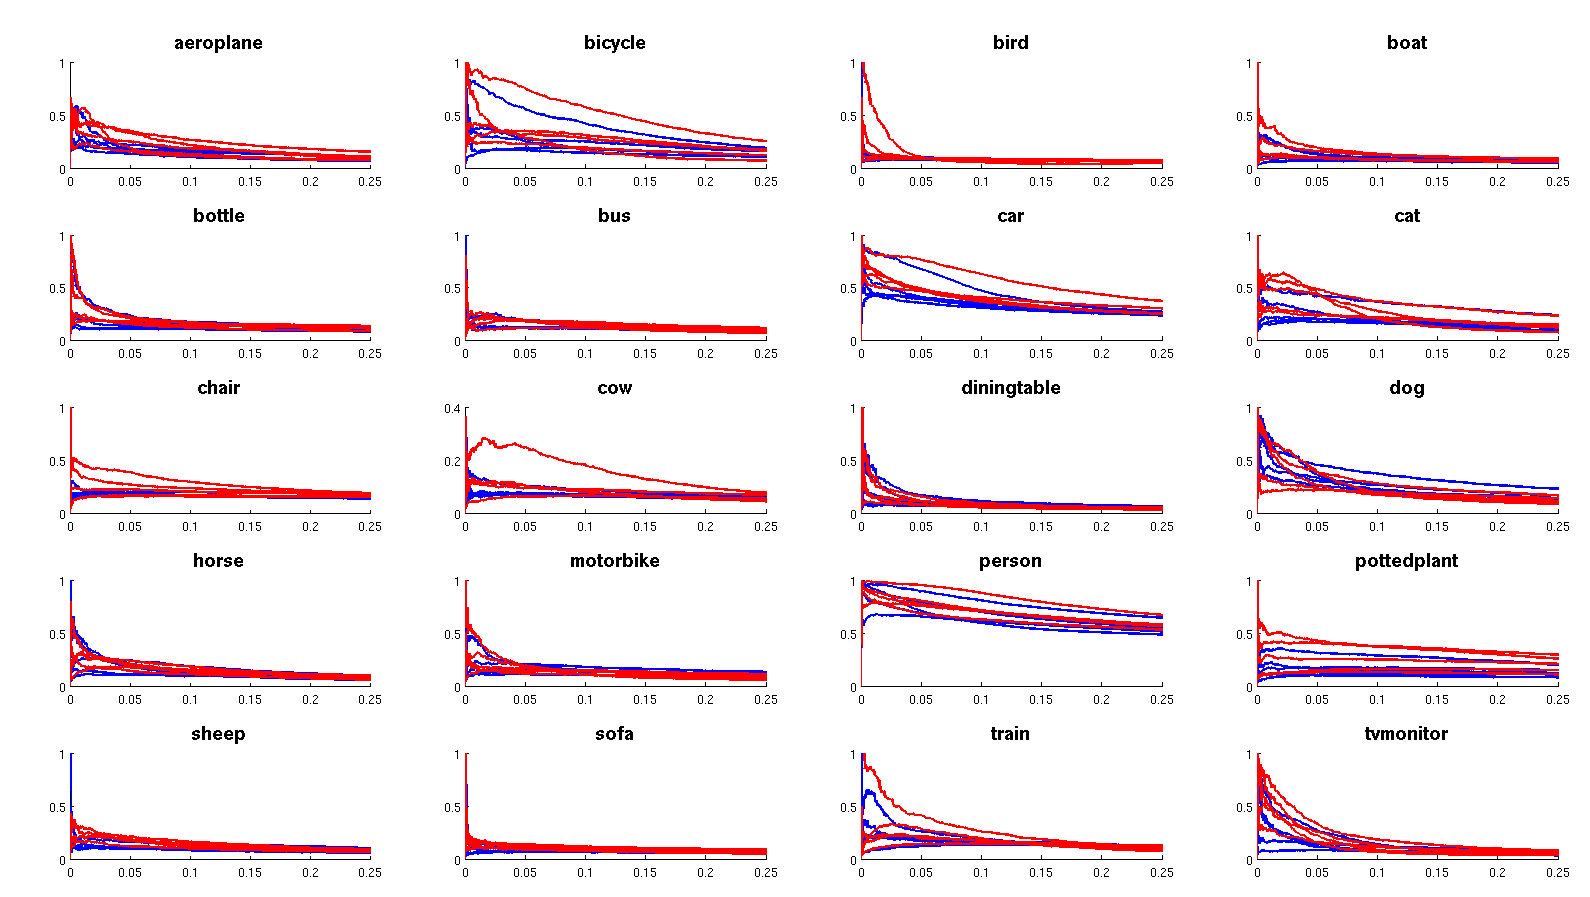
\includegraphics[scale=0.20]{images/gtbbox_pascal_prerec_pool5units.png}}
\caption{Precision-Recall Curves for 20 PASCAL Classes calculated using pool-5 filter responses on ground truth bounding boxes. Red-Curves: Fine Tuned Network, Blue-Curves: Alex-Net. The figure only displays 5 best filters for each class based on AP  upto a recall threshold of 0.25. For most classes, precision drops significantly even at modest recall values.}
\label{fig:ap}
\end{figure}

%\begin{figure}[t!]
%\centering
%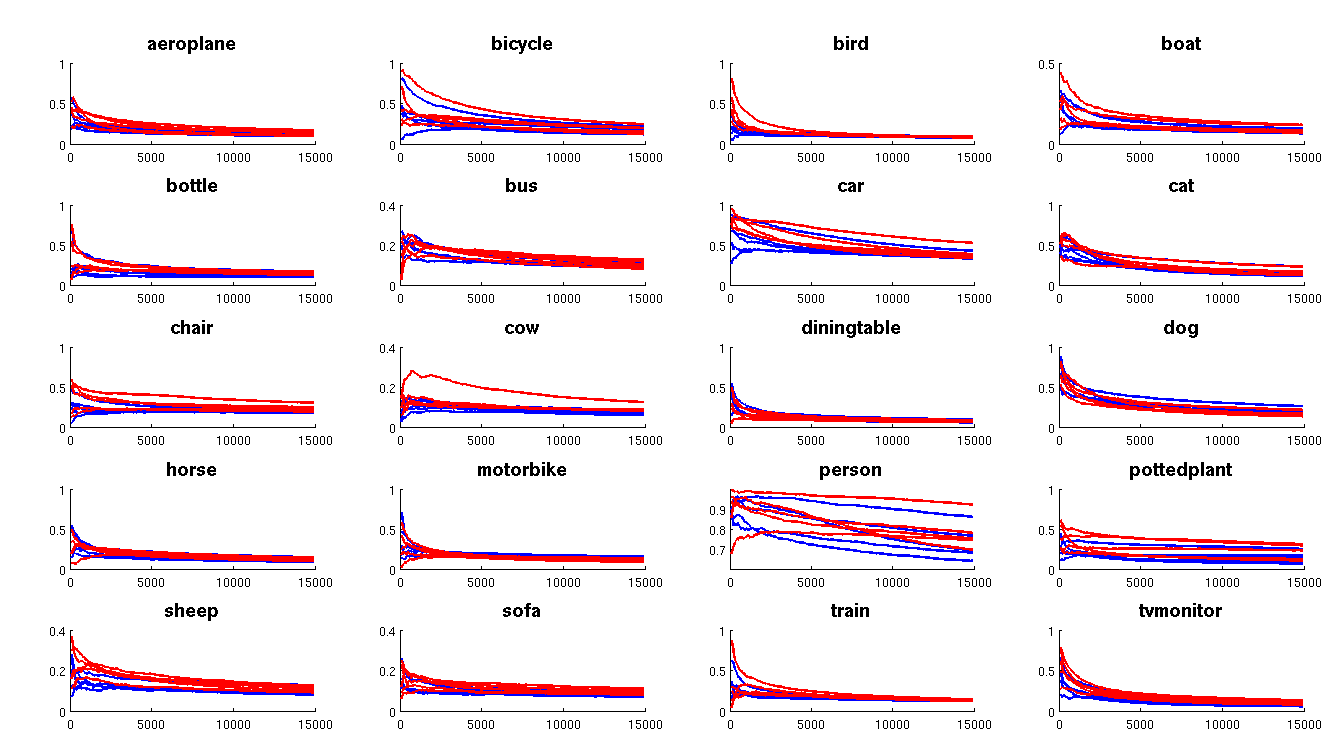
\includegraphics[scale=0.20]{images/prob_sel_dims_top5.png}
%\caption{This plot shows the precision curve for the top 5 most selective filters taken from Alex-Net (Blue) and FT-Net(Red) for all PASCAL classes. Y-axis is the precision and X-axis is number of examples.}
%\label{fig:prob-sel}
%\end{figure}

\subsection{How many filters are required for discrimination?}
\label{sub:how-many}
In order to answer this question we train linear a svm for each class using only a subset of 256 pool-5 filters. In particular we construct subsets of size k, where k takes the values - [1,2,3,5,10,15,20,25,30,35,40,45, \newline 50,80, 100,128,256]. A subset of size k is constructed independently for each class using a greedy selection strategy described in figure \ref{fig:sel-strategy}. We use the variation in performance with the number of filters needed as a metric to evaluate how many filters are needed for each class. 
  
\begin{figure}[t!]
\centering
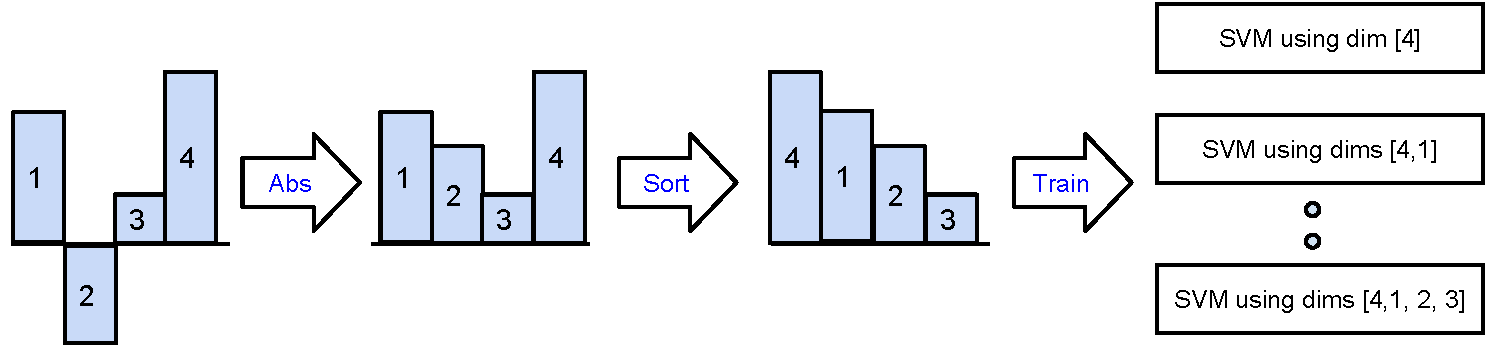
\includegraphics[scale=0.35]{images/how-many.pdf}
\caption{Illustration of our greedy strategy for constructing subsets of filters. For each class we first train a linear-svm using the spatial-max feature transformation described in section \ref{sub:imp-loc}. Spatial-max leaves us with a 256-D vector wherein each dimension has a one to one correspondence with 256 pool-5 filters. We use the magnitude of each dimension of the learnt weight vector as a proxy for the importance of that dimension towards discriminating a given class. For the purpose of illustration we describe the procedure with a 4-D weight vector shown on the extreme left (the numbers on each bar are the "dimension"). Firstly, we take the absolute value for each dimension and then sort the dimensions based on this value. Then, we chose the top k filters/dimensions from this ranked list to construct a subset of size k.}
\label{fig:sel-strategy}
\end{figure}

The results of our analysis are summarized in fig \ref{fig:svm-sel-dims} and table \ref{table:num-fil}. For classes such as persons, cars, cats we require a relatively few number of filters, but for most of the classes we need to look at around 30-40 filters to achieve atleast 90\% of the full performance. This also indicates, that for a few classes yes, there are grand-mother kind of neurons but for a lot of classes the representation is distributed. Also, as expected the fine-tuned network requires activations of a fewer numbers of filters to achieve the same performance but this reduction in number of filters is not large. 

\begin{figure}[t!]
\centering
%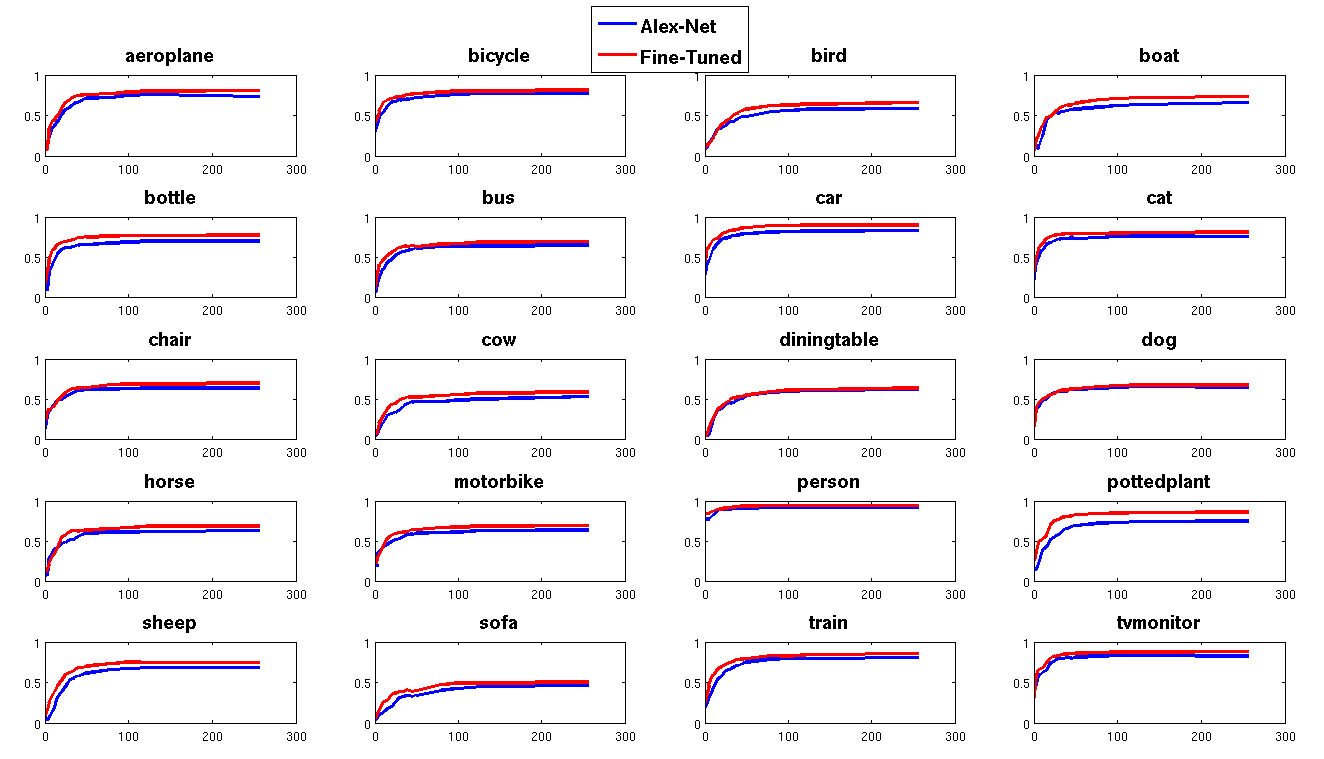
\includegraphics[height=6.5cm]{images/svm_seldims.png}
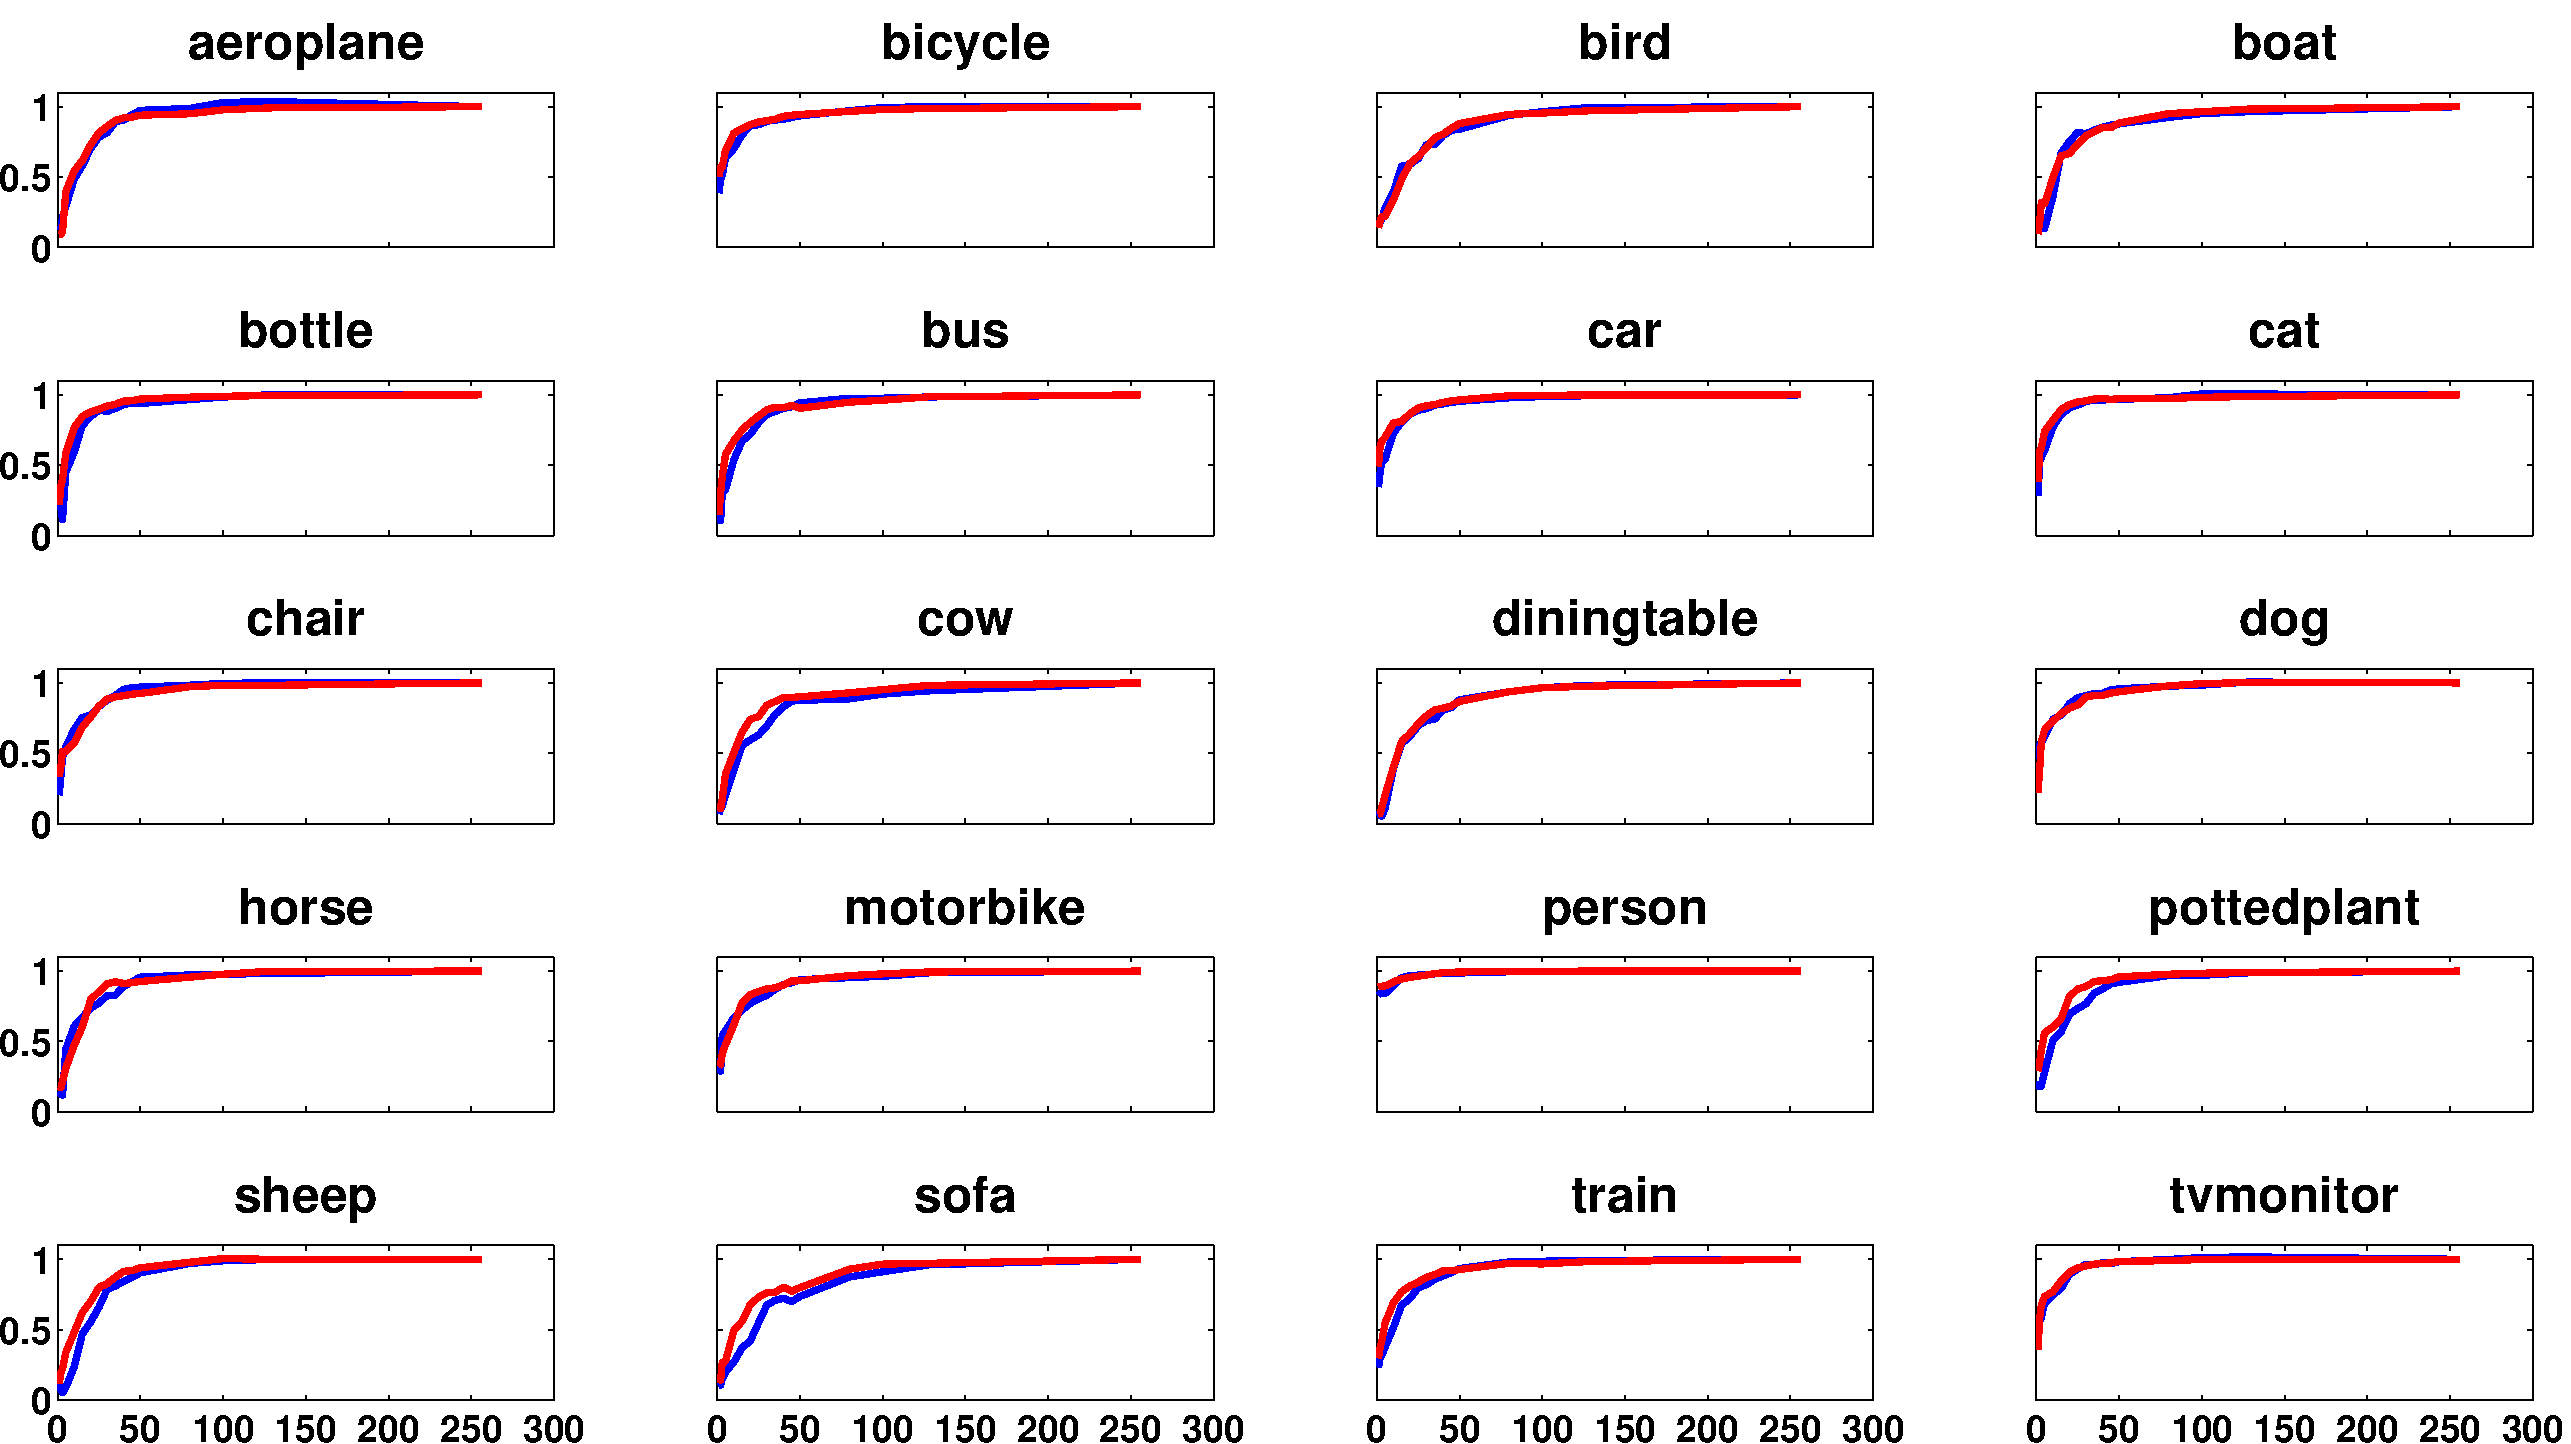
\includegraphics[height=6.5cm]{images/pool5_spmax_num_svm_filters.pdf}
\caption{Analysis of how many filters are required to classify ground truth bounding boxes for 20 categories taken from PASCAL-2007 detection challenge. The y-axis in each of plot represents classification accuracy measured as mean-ap where as x-axis stand for the number of filters.)}
\label{fig:svm-sel-dims}
\end{figure}



\setlength{\tabcolsep}{1pt}
\begin{table}[t!]
\begin{center}
\caption{Number of filters required to achieve 50\% ,90\% of the full performance for PASCAL classes using Alex-Net(AN) and the Fine-Tuned network(FT)}
\label{table:num-fil}
\tiny
\begin{tabular}{lc||cccccccccccccccccccc}
\hline\noalign{\smallskip}
Net & AP & aero & bike & bird & boat & bottle & bus & car & cat & chair & cow & table & dog & horse & mbike & person & plant & sheep & sofa & train & tv \\
\noalign{\smallskip}
\hline
AN & 50 & 15 & 3 & 15 & 15 & 10 & 10 & 3 & 2 & 5 & 15 & 15 & 2 & 10 & 3 & 1 & 10 & 20 & 25 & 10 & 2 \\ 
FT & 50 & 10 & 1 & 20 & 15 & 5 & 5 & 2 & 2 & 3 & 10 & 15 & 3 & 15 & 10 & 1 & 5 & 15 & 15 & 5 & 2 \\
\hline
\noalign{\smallskip}
AN & 90 & 40 & 35 & 80 & 80 & 35 & 40 & 30 & 20 & 35 & 100 & 80 & 30 & 45 & 40 & 15 & 45 & 50 & 100 & 45 & 25 \\
FT & 90 & 35 & 30 & 80 & 80 & 30 & 35 & 25 & 20 & 35 & 50 & 80 & 35 & 30 & 40 & 10 & 35 & 40 & 80 & 40 & 20 \\
\hline
\end{tabular}
\end{center}
\end{table}
\setlength{\tabcolsep}{1.4pt}

\begin{figure}[t!]
\centering
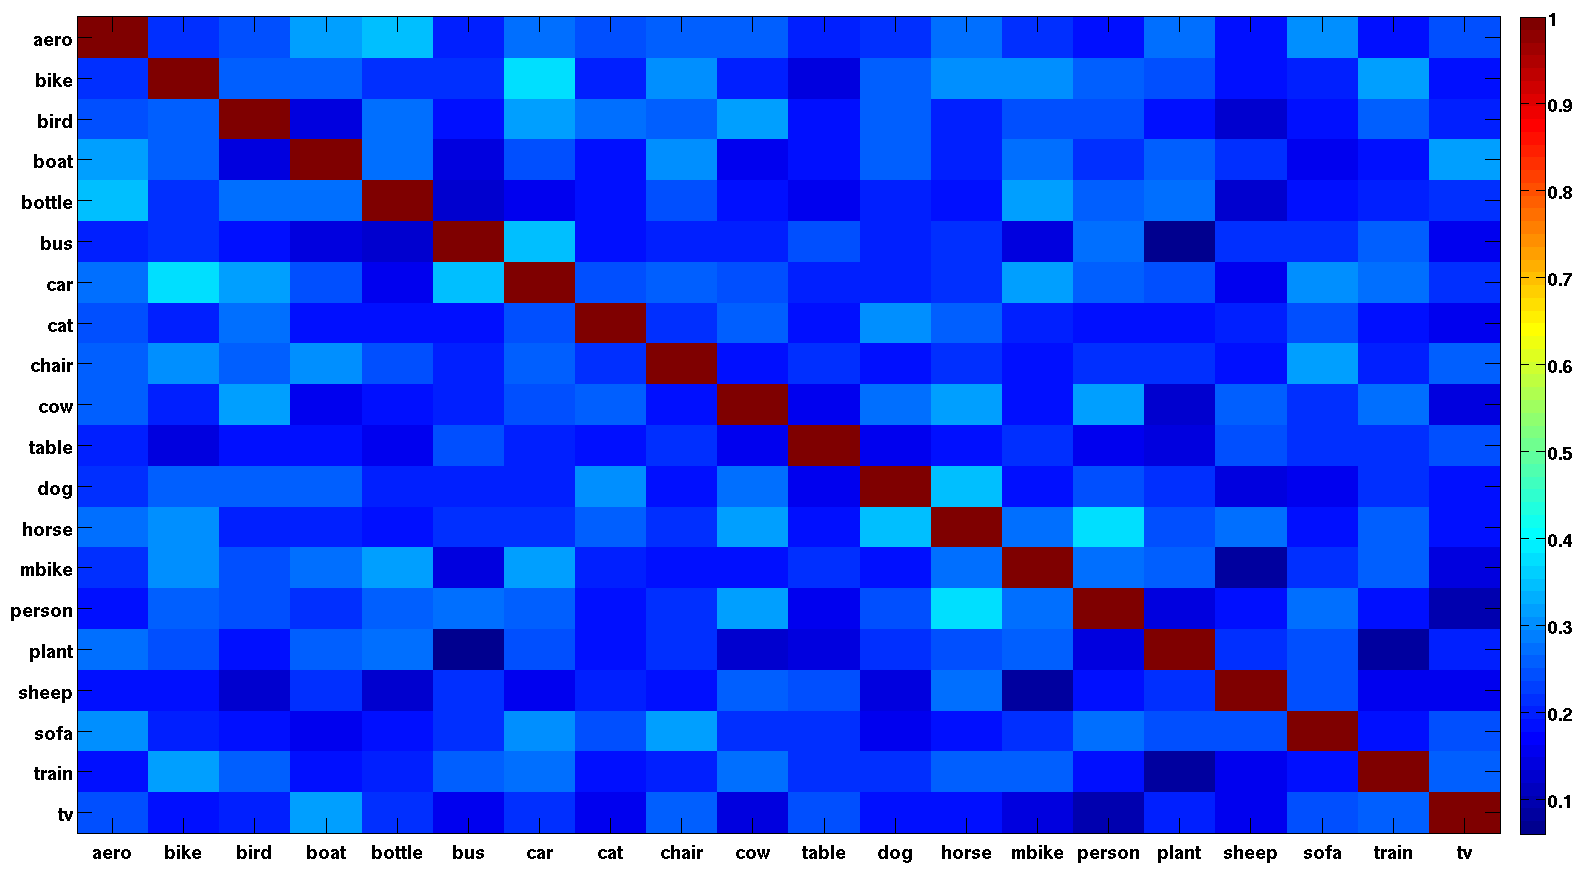
\includegraphics[width=1.0\linewidth]{images/ftNet_commonfilters.png}
\caption{This plot depicts the degree of overlap among the top-50 filters in layer 5 of
finetuned network used for classifying each category of the PASCAL 2007 challenge. Entry
(i,j) of the matrix is the fraction of filters of the i th class which are common with j th class. This plot indicates, that there is very little overlap between filters used for different classes.}
\label{fig:svm-sel-dims}
\end{figure}




\subsection{Discussion}
%Although in our analysis we find that for discriminating some classes only a few units suffice whereas for others quite a lot of them are required. 
%The ''extent" to which the code is distributed is likely to be a function of number of filters. If there are a few filters we will expect the code to be more distributed whereas if there are a large number of filters we expect to find more Grandmother kind of cells. The other important tradeoffs to consider are accuracy and training time as a function of number of filters in each layer. We as a community have only had a chance to experiment with a few network architectures out of the exponentially large number of possibilities. Although, it is beyond the scope of the current work determining the optimal number of filters in each layer is an open important question which needs to be addressed! 
To include somewhere: It is also notable to point out that the more or less generic representations learnt in layer 4 and 5 are in contrast with some of the mid-level feature learning work such as \cite{Blocks} \cite{Mid1} wherein the problem of finding good mid-level parts is often posed as a greedy search for high recall discriminative templates.


